%---------------------------------------------------------------------
\subsection{Bibliometria}\label{metodologiaBibliometria}
%---------------------------------------------------------------------

A \autoref{tab_bibliometria_termosInformationConfig} contém dados bibliométricos
de pesquisas de termos chaves em algumas das bases de dados listadas na
\autoref{metodologiaFontes}\ldots

% EXEMPLO DE LONG TABLE
% INFORMATION e CONFIGURATION - Tabela principal de consultas de
\begin{center}
\footnotesize{
\begin{ThreePartTable}

\begin{longtable}{p{7.2cm}|p{6.3cm}|p{1.8cm}}

\caption[Resultados obtidos na consulta de termos ``configuration'' e
``information'' em bases de dados em 29.1.2012.]{\footnotesize{Resultados obtidos
na consulta de termos ``configuration'' e ``information'' em bases de dados.
Consultas realizadas em 29.1.2012. Período pesquisado: todos disponíveis nas
bases.}}
\label{tab_bibliometria_termosInformationConfig}
\\

%This is the header for the first page of the table...
\hline 
\textbf{Base de dados}	& \textbf{Termos e critérios} & \textbf{Resultados} \\
\hline 
%\endfirsthead
\endhead

%This is the footer for all pages except the last page of the table...
  \multicolumn{3}{r}{{Continua\ldots\ldots}} \\
\endfoot

%This is the footer for the last page of the table...
\hline \hline
\endlastfoot

%Now the data...

    % ``information configuration''
	\multirow{2}{*}{Academic Search Premier - ASP (EBSCO)}\tnote{a}
	& Titulo=(``information configuration'')
	& 1\tnote{b}
	\\
	& Titulo=(``configuration of information'')
	& 1\tnote{e}	
	\\ \hline	

	\multirow{2}{*}{Cambridge Journals Online}\tnote{a}
	& Titulo=(``information configuration'')
	& 0
	\\
	& Titulo=(``configuration of information'')
	& 0
	\\ \hline	

	\multirow{2}{*}{Highwire Press}\tnote{a}
	& Titulo=(``information configuration'')
	& 0
	\\
	& Titulo=(``configuration of information'')
	& 0
	\\ \hline	

	\multirow{2}{*}{Nature (NPG)}\tnote{a}
	& Titulo=(``information configuration'')
	& 0
	\\
	& Titulo=(``configuration of information'')
	& 0
	\\ \hline	

	\multirow{2}{*}{Oxford Journals (Oxford University Press)}\tnote{a}
	& Titulo=(``information configuration'')
	& 0
	\\
	& Titulo=(``configuration of information'')
	& 0
	\\ \hline	

	\multirow{3}{*}{SciELO.ORG}\tnote{a}
	& Titulo=(``information configuration'')
	& 0
	\\
	& Titulo=(``configuration of information'')
	& 0
	\\
	& Title: ``configuração da informação''
	& 0
	\\ \hline	

	\multirow{2}{*}{Science (AAAS)}\tnote{a}
	& Titulo=(``information configuration'')
	& 0
	\\
	& Titulo=(``configuration of information'')
	& 0
	\\ \hline	

	\multirow{2}{*}{ScienceDirect (Elsevier)}\tnote{a}
	& Titulo=(``information configuration'')
	& 0
	\\
	& Titulo=(``configuration of information'')
	& 0
	\\ \hline	

	\multirow{2}{*}{SpringerLink (MetaPress)}\tnote{a}
	& Titulo=(``information configuration'')
	& 0
	\\
	& Titulo=(``configuration of information'')
	& 0
	\\ \hline	

	\multirow{2}{*}{E-LIS}
	& Title: ``information configuration''
	& 2\tnote{c}
	\\
	& Title: ``configuration of information''
	& 1\tnote{d}
	\\ \hline	

	\multirow{2}{*}{Web of Knowledge}
	& Title: ``information configuration''
	& 0
	\\
	& Title: ``configuration of information''
	& 0
	\\ \hline	
	
\end{longtable}

	\begin{tablenotes}
		\item [a] Base de Periódicos CAPES.
		\item [b] O único texto obtido \ldots
		\item [c] Os textos recuperados \cite{hammer2005} e \cite{apps2001} se
		referem, respectivamente, a um manual de uso de uma ferramenta de
		gerenciamento de informação para bibliotecários e a um serviço baseado em Dublincore.
		\item [d] O único texto obtido \ldots
		\item [e] O único texto obtido \ldots

	\end{tablenotes}
	
\end{ThreePartTable}
}
\end{center}


% Figura - Web of Science 1 - Detalhamento
\begin{figure}[htb]
\begin{center}
  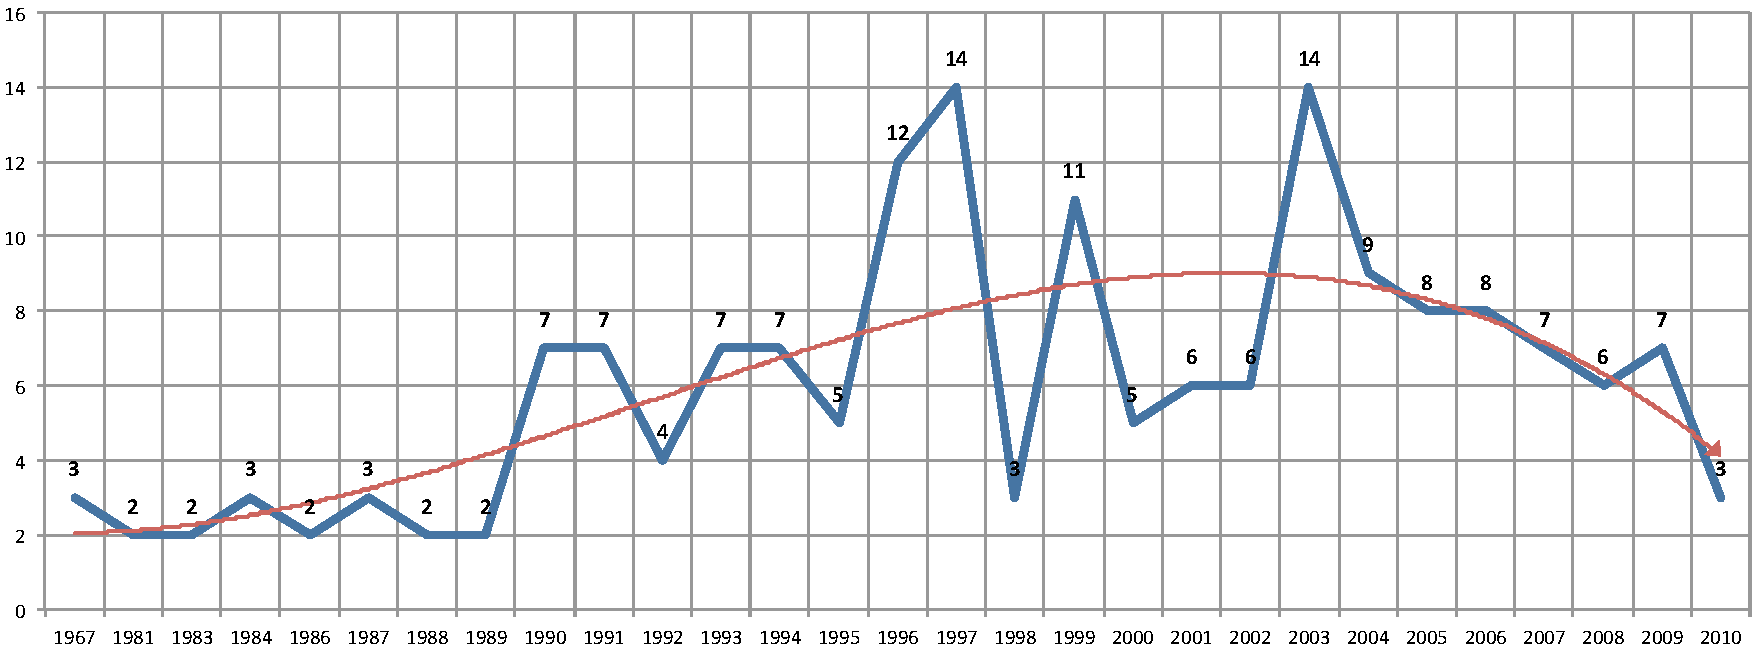
\includegraphics[scale=0.55]{imagens/bibliometriaWebOfScience1.pdf}
  \caption{\label{fig_biblioWebOfScience1}Bibliometria - Web of Science -
  Detalhamento da consulta - Critério: Title=(``configuration management'').}
  \caption*{Fonte: autores}
\end{center}
\end{figure}

